\documentclass[12pt, twoside]{article}
\usepackage[letterpaper, margin=1in, headsep=0.5in]{geometry}
\usepackage[english]{babel}
\usepackage[utf8]{inputenc}
\usepackage{amsmath}
\usepackage{amsfonts}
\usepackage{amssymb}
\usepackage{tikz}
\usetikzlibrary{quotes, angles}
\usepackage{graphicx}
\usepackage{multicol}

%\usepackage{pgfplots}
%\pgfplotsset{width=10cm,compat=1.9}
%\usepgfplotslibrary{statistics}
%\usepackage{pgfplotstable}
%\usepackage{tkz-fct}
%\usepackage{venndiagram}

\usepackage{fancyhdr}
\pagestyle{fancy}
\fancyhf{}
\renewcommand{\headrulewidth}{0pt} % disable the underline of the header

\fancyhead[RE]{\thepage}
\fancyhead[RO]{\thepage \\ Name: \hspace{3cm}}
\fancyhead[L]{BECA / Dr. Huson / Geometry 10th Grade\\* Unit 1: Introduction to Geometry\\23 September 2019}

\begin{document}
\subsubsection*{2.6 Homework: Areas of squares and compound shapes}
  \vspace{0.25cm}
  \begin{enumerate}


    \item Construction a line perpendicular to $\overleftrightarrow{EF}$ through the point $G$. \vspace{5cm}
      \begin{center}
      \begin{tikzpicture}
        \draw [<->, thick] (0,0)--(10,0);
        \draw [fill] (1,0) circle [radius=0.05] node[below]{$E$};
        \draw [fill] (8,0) circle [radius=0.05] node[below]{$F$};
        \draw [fill] (5,1) circle [radius=0.05] node[below right]{$G$};
      \end{tikzpicture}
      \end{center} \vspace{4cm}

      \item Accurately draw and label a square with sides of length 3 centimeters. Find the area of the square. \vspace{6cm}
      
      \item The area of a square is 81 square centimeters. Find the length of the side of the square.

    \newpage

    \item Find the combined area of the shape shown below, a rectangle and a square. The grid is in centimeters.
    \begin{flushleft}
      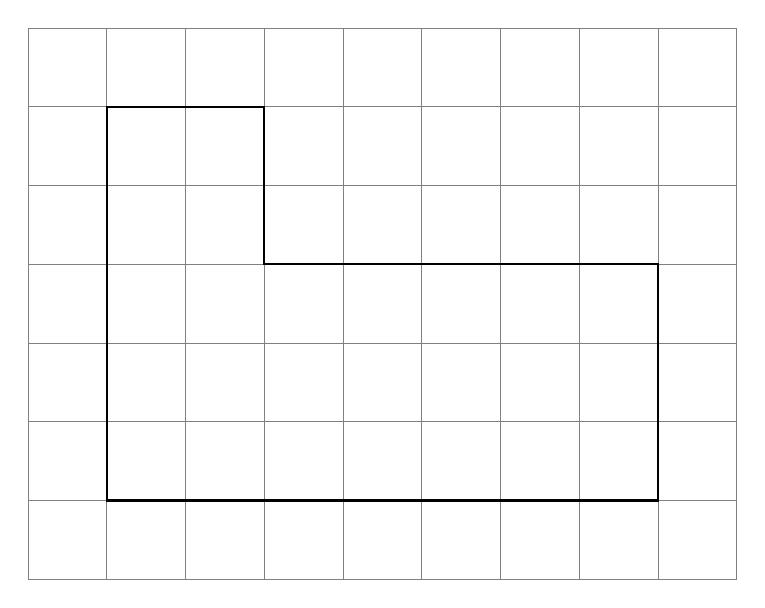
\begin{tikzpicture}[scale=1]
        \draw [help lines] (-4,-4) grid (5,3);
        %\draw [thick, ->] (-2.2,0) -- (10.4,0) node [below right] {$x$};
        %\draw [thick, ->] (0,-2.2)--(0,10.4) node [left] {$y$};
        %\draw (0,0) circle [radius=3] node[below]{$C$};
        %\draw [fill] (0,0) circle [radius=0.05];
        \draw [thick, -] (-3,-3)--(4,-3)--(4,0)--(-1,0)--(-1,2)--(-3,2)--cycle;
      \end{tikzpicture}
    \end{flushleft} \vspace{1cm} 

    \item The compound shape shown below is composed of a square with side length 5 cm and a triangle with base 2 cm. Find the total area of the combined shape.
    \vspace{1cm} 
    \begin{flushleft}
    \begin{tikzpicture}
      \draw [-, thick] (0,0)--(7,0)--(5,5)--(0,5)--cycle;
      \draw [dashed] (5,0)--(5,5);
      %\draw [fill] (0,0) circle [radius=0.05] node[left]{$A$};
      %\draw [fill] (7,0) circle [radius=0.05] node[right]{$B$};
      %\draw [fill] (7,2) circle [radius=0.05] node[right]{$C$};
      %\draw [fill] (0,2) circle [radius=0.05] node[left]{$D$};
      \node at (6, -0.5){2};
      \node at (2.5, -0.5){5};
      \node at (-0.5, 2.5){5};
    \end{tikzpicture}
    \end{flushleft} \vspace{1cm}  

   
  \end{enumerate}
\end{document}
